% **************************************************
% Document Class Definition
% **************************************************
\documentclass[%
	paper=A4,					% paper size --> A4 is default in Germany
	twoside=true,				% onesite or twoside printing
	openright,					% doublepage cleaning ends up right side
	parskip=full,				% spacing value / method for paragraphs
	chapterprefix=true,			% prefix for chapter marks
	11pt,						% font size
	headings=normal,			% size of headings
	bibliography=totoc,			% include bib in toc
	listof=totoc,				% include listof entries in toc
	titlepage=on,				% own page for each title page
	captions=tableabove,		% display table captions above the float env
	draft=false,				% value for draft version
]{scrreprt}%

% **************************************************
% Debug LaTeX Information
% **************************************************
%\listfiles

% **************************************************
% Information and Commands for Reuse
% **************************************************
\newcommand{\thesisTitle}{Big Master Project}
\newcommand{\thesisName}{The Haptic Printer}

\newcommand{\thesisDate}{September 27, 2021}
\newcommand{\thesisVersion}{Final}

\newcommand{\departmentHead}{Prof. Dr. Jörg Müller}
% \newcommand{\thesisFirstReviewerUniversity}{\protect{Universit{\"a}t Bayreuth}}
% \newcommand{\thesisFirstReviewerDepartment}{Fakult{\"a}t Mathematik, Physik, Informatik}

% \newcommand{\thesisSecondReviewer}{Dr. Stefan Sch{\"o}nig}
% \newcommand{\thesisSecondReviewerUniversity}{\protect{Universit{\"a}t Bayreuth}}
% \newcommand{\thesisSecondReviewerDepartment}{Fakult{\"a}t Mathematik, Physik, Informatik}

\newcommand{\thesisFirstSupervisor}{Viktorija Paneva}
% \newcommand{\thesisSecondSupervisor}{Lars Ackermann}

\newcommand{\thesisUniversity}{\protect{Universit{\"a}t Bayreuth}}
\newcommand{\thesisUniversityDepartment}{Fakult{\"a}t Mathematik, Physik, Informatik}
\newcommand{\thesisUniversityInstitute}{Institut f{\"u}r Informatik}
\newcommand{\thesisUniversityGroup}{Lehrstuhl für Serious Games}
\newcommand{\thesisUniversityCity}{Bayreuth}
\newcommand{\thesisUniversityStreetAddress}{Universit{\"a}tsstrasse 30}
\newcommand{\thesisUniversityPostalCode}{95447}

% **************************************************
% Load and Configure Packages
% **************************************************
\usepackage[utf8]{inputenc}		% defines file's character encoding
\usepackage[english]{babel} % babel system, adjust the language of the content
\usepackage{float}       % helps in image position fix
\usepackage[					% clean thesis style
	figuresep=colon,%
	sansserif=false,%
	hangfigurecaption=false,%
	hangsection=true,%
	hangsubsection=true,%
	colorize=full,%
	colortheme=bluemagenta,%
	bibsys=bibtex,%
	bibfile=bib-refs,%
	bibstyle=alphabetic,%
]{cleanthesis}

\usepackage{listings}
\usepackage{xcolor}

\definecolor{codegreen}{rgb}{0,0.6,0}
\definecolor{codegray}{rgb}{0.5,0.5,0.5}
\definecolor{codepurple}{rgb}{0.58,0,0.82}
\definecolor{backcolour}{rgb}{0.95,0.95,0.92}

\lstdefinestyle{mystyle}{
	backgroundcolor=\color{backcolour},   
	commentstyle=\color{codegreen},
	keywordstyle=\color{magenta},
	numberstyle=\tiny\color{codegray},
	stringstyle=\color{codepurple},
	basicstyle=\ttfamily\footnotesize,
	breakatwhitespace=false,         
	breaklines=true,                 
	captionpos=b,                    
	keepspaces=true,                 
	numbers=left,                    
	numbersep=5pt,                  
	showspaces=false,                
	showstringspaces=false,
	showtabs=false,             
	tabsize=2
}

\lstset{style=mystyle}


\hypersetup{					% setup the hyperref-package options
	pdftitle={\thesisTitle},	% 	- title (PDF meta)
	pdfauthor={\thesisName},	% 	- author (PDF meta)
	plainpages=false,			% 	-
	colorlinks=false,			% 	- colorize links?
	pdfborder={0 0 0},			% 	-
	breaklinks=true,			% 	- allow line break inside links
	bookmarksnumbered=true,		%
	bookmarksopen=true			%
}


% **************************************************
% Document CONTENT
% **************************************************
\begin{document}

% --------------------------
% rename document parts
% --------------------------
%\renewcaptionname{ngerman}{\figurename}{Abb.}
%\renewcaptionname{ngerman}{\tablename}{Tab.}
\renewcaptionname{english}{\figurename}{Fig.}
\renewcaptionname{english}{\tablename}{Tab.}

% --------------------------
% Front matter
% --------------------------
\pagenumbering{roman}			% roman page numbing (invisible for empty page style)
\pagestyle{empty}				% no header or footers
% !TEX root = ../The-Haptic-Printer.tex
%
% ------------------------------------  --> cover title page
\begin{titlepage}
	\pdfbookmark[0]{Cover}{Cover}
	\includegraphics[width=8cm]{gfx/Universität_Bayreuth} \\[2mm]
	\textsf{\thesisUniversityDepartment} \\
	\textsf{\thesisUniversityInstitute} \\
	\textsf{\thesisUniversityGroup} \\
	\textsf{\departmentHead}

		\flushright
	\vfill
	{\LARGE\thesisTitle \par}
	\rule[5pt]{\textwidth}{.4pt} \par
	\textbf{\Large\thesisName}
	\vfill
	\begin{flushleft}
		Author : \textbf{Anuj Sharma}, \\
		\hspace*{1.5cm}\textbf{Akshaya Kumar Krishnappa Ramakrishna}\\[2mm]
		Supervisor : \textbf{\thesisFirstSupervisor}
	\end{flushleft}
	\rule[5pt]{\textwidth}{.4pt} \par
	\textit{\large\thesisDate} \\
	Version: \thesisVersion
\end{titlepage}
		% INCLUDE: all titlepages
\cleardoublepage

\pagestyle{plain}				% display just page numbers
% !TEX root = ../The-Haptic-Printer.tex
%
\pdfbookmark[0]{Abstract}{Abstract}
\chapter*{Abstract}
\label{sec:abstract}
\vspace*{-10mm}
Over the years of evolution of human computer interaction, we have seen various kinds of interaction techniques. The recent trend of contactless haptic technology has been on the rise. In our project we focus on rendering custom shapes on the user palm, using different kinds of rendering techniques. The main objective of this project is to map various kinds of user input like CSV, SVG, drawing from canvas and inputs from leap motion. We consume these inputs and process them in order to render custom shapes. Also, this report analyses and compares the different techniques of rendering with various validation techniques and deduces an overall result from the study and implementation of the proposed application.



		% INCLUDE: the abstracts (english and german)
\cleardoublepage
%
\cleardoublepage
%
\setcounter{tocdepth}{2}		% define depth of toc
\tableofcontents				% display table of contents
\cleardoublepage

% --------------------------
% Body matter
% --------------------------
\pagenumbering{arabic}			% arabic page numbering
\setcounter{page}{1}			% set page counter
\pagestyle{maincontentstyle} 	% fancy header and footer

% !TEX root = ../The-Haptic-Printer.tex
%
\chapter{Introduction}
\label{sec:intro}

The haptic technology enables human computer interaction in a new way compared to previous existent interaction techniques. Haptics gives us a new dimension of interaction technique without any physical contact between the user and the device. This contactless haptic technologies give rise to various kind of applications in real life scenarios. One prominent among them is the mid air user interfaces, where the use of hand and finger movements are used to control the interface. Ultrasound haptic technology \cite{iwamoto2008non} is one of the example of contactless haptic technology where ultrasound waves are emitted by the device and coincide at a particular point in space to give haptic sensations. 


\section{About Ultrahaptics}
\label{sec:intro:about ultrahaptics}


The human skin has mechanoreceptors which are sensory cells that convert mechanical forces into nerve excitation. When the sound waves make contact with the skin, it gives a tactile sensation for the user. In order to produce such ultrasound waves we make use of a device manufactured by Ultraleap \cite{ul} called as Ultrahaptics.	The device emits ultrasound from its phased array which propagates as a wave with a frequency higher than the limit of human hearing. Each emitter in the device emits the wave and every wave emitted coincide at a point in the air. This coincidence of the waves at a point is called a focal point and this focal point when directed towards a user palm creates a pressure for the user and the user can perceive it as a tactile sensation. The coincidence of waves at a focal point, strength and intensity of each transducer is handled by the Ultrahaptics device itself by using various solver algorithms.

In order to render custom shapes we need to explore various techniques of rendering and experiment with different parameters of the device. The different parameters available in the device are intensity, frequency, multiple focal points and the different techniques of rendering are explained in the next section of literature survey. 

\section{Project objective}
\label{sec:intro:objective}

Using the concept of mid air interfaces, we can explore and build many applications in real world. In the recent times due to the COVID-19 pandemic, one prominent use case would be to build contactless interfaces in the public space. In order to achieve this we need to render custom shapes to the user in order to make user aware of different kinds of sensation.
In this project, our main focus is to render custom shapes on user's palm using different kinds of inputs. Here, different kinds of inputs means different various formats like CSV (comma-separated values), SVG (Scalable Vector Graphics), user drawing and Leap Motion. We process all these kind of inputs and render the dynamic shapes using the Ultrahaptics device. 

 % INCLUDE: introduction
% !TEX root = ../The-Haptic-Printer.tex
%
\chapter{Literature Survey}
\label{sec:related}

Once our project objective was clear we had to find out existing rendering techniques available for Ultrahaptics device. Also, we had to look into Ultrahatics Software Development Kit (SDK) and the available Application Program Interface (API) so that the application can be developed. After referring to Ultrahaptics SDK we came to know that there are two techniques available to develop our application, namely Amplitude Modulation (AM) and Time Point Streaming(TPS). To further understand these topics we had to look into the concepts and working of these techniques. So we did a literature survey and in the further subsection we have listed our key findings and short explanation of both the techniques.

\begin{figure}[htb]
	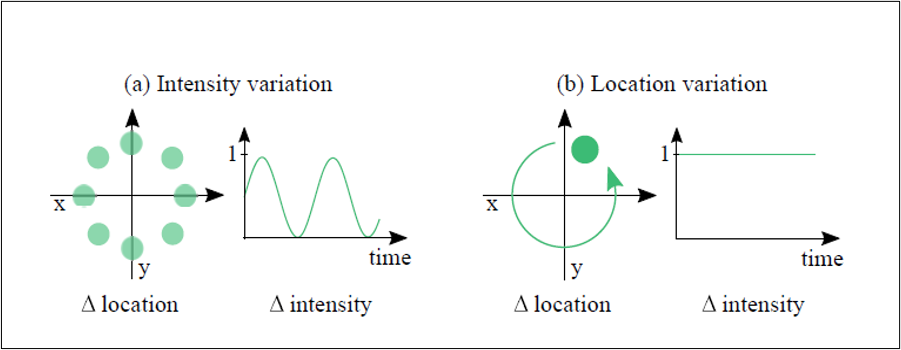
\includegraphics[width=\textwidth]{gfx/am_tps.png}
	\caption{(a) shows working of Amplitude Modulation technique (b) shows working of Spatiotemporal Modulation technique \cite{Frier2018}}
	\label{fig:related:am_tps}
\end{figure}

\section{Amplitude Modulation}
\label{sec:related:sec1}

In amplitude modulation technique, the ultrasound waves emitted by the phased arrays and are modulated by switching them off and then on again fast enough to stimulate the vibration-sensitive touch receptors (mechanoreceptors) in the skin of the hands, giving tactile sensation. But these switching on and off of waves are not so easily perceived by the user as the frequencies are in the range of 40Hz to 400Hz. In order to smoothen out this effect the ultrasound is modulated with a sinusoidal wave.\cite{am}

As shown in Fig 2.1 (a) the control points have varying intensity emitted by the device which creates pressure points on user's palm. Using this technique, we can render shapes by updating the coordinates of  the shape rapidly. Also, we can use one more technique here by emitting multiple control points at the same time to complete the shape outline.


\section{Spatiotemporal Modulation}
\label{sec:related:sec2}

Spatiotemporal Modulation also called as time point streaming is a technique where we rapidly move the control point emitted by the device along the shape outline to create tactile sensation. Here the control point can be fixed to a same intensity level or we can use any sine or cosine wave as intensity values for varying intensities.\cite{tps} 

As shown in Fig 2.1 (b) the control point moves rapidly along the circle shape outline with constant intensity. 

Once we discovered the various techniques available in Ultrahaptics SDK we decided to go ahead with these two techniques. There are several tweaks available to these two techniques which can also be used for rendering. However, due to the limitation of available Ultrahaptics SDK API we chose to stick to these two techniques.  

 % INCLUDE: related work
% !TEX root = ../The-Haptic-Printer.tex
%
\chapter{Features}
\label{sec:concepts}

\cleanchapterquote{A good end product is not just a collection of features, Its how it all works together.}{Tim Cook}{-CEO Apple Inc.}

As mentioned previously the main objective of the application is to consume multiple types of 
inputs from user and render it to the 
Ultrahaptics device. The features are built keeping those multiple inputs in mind. 
A display of multiple inputs can be seen in the image below.
\begin{figure}[htb]
	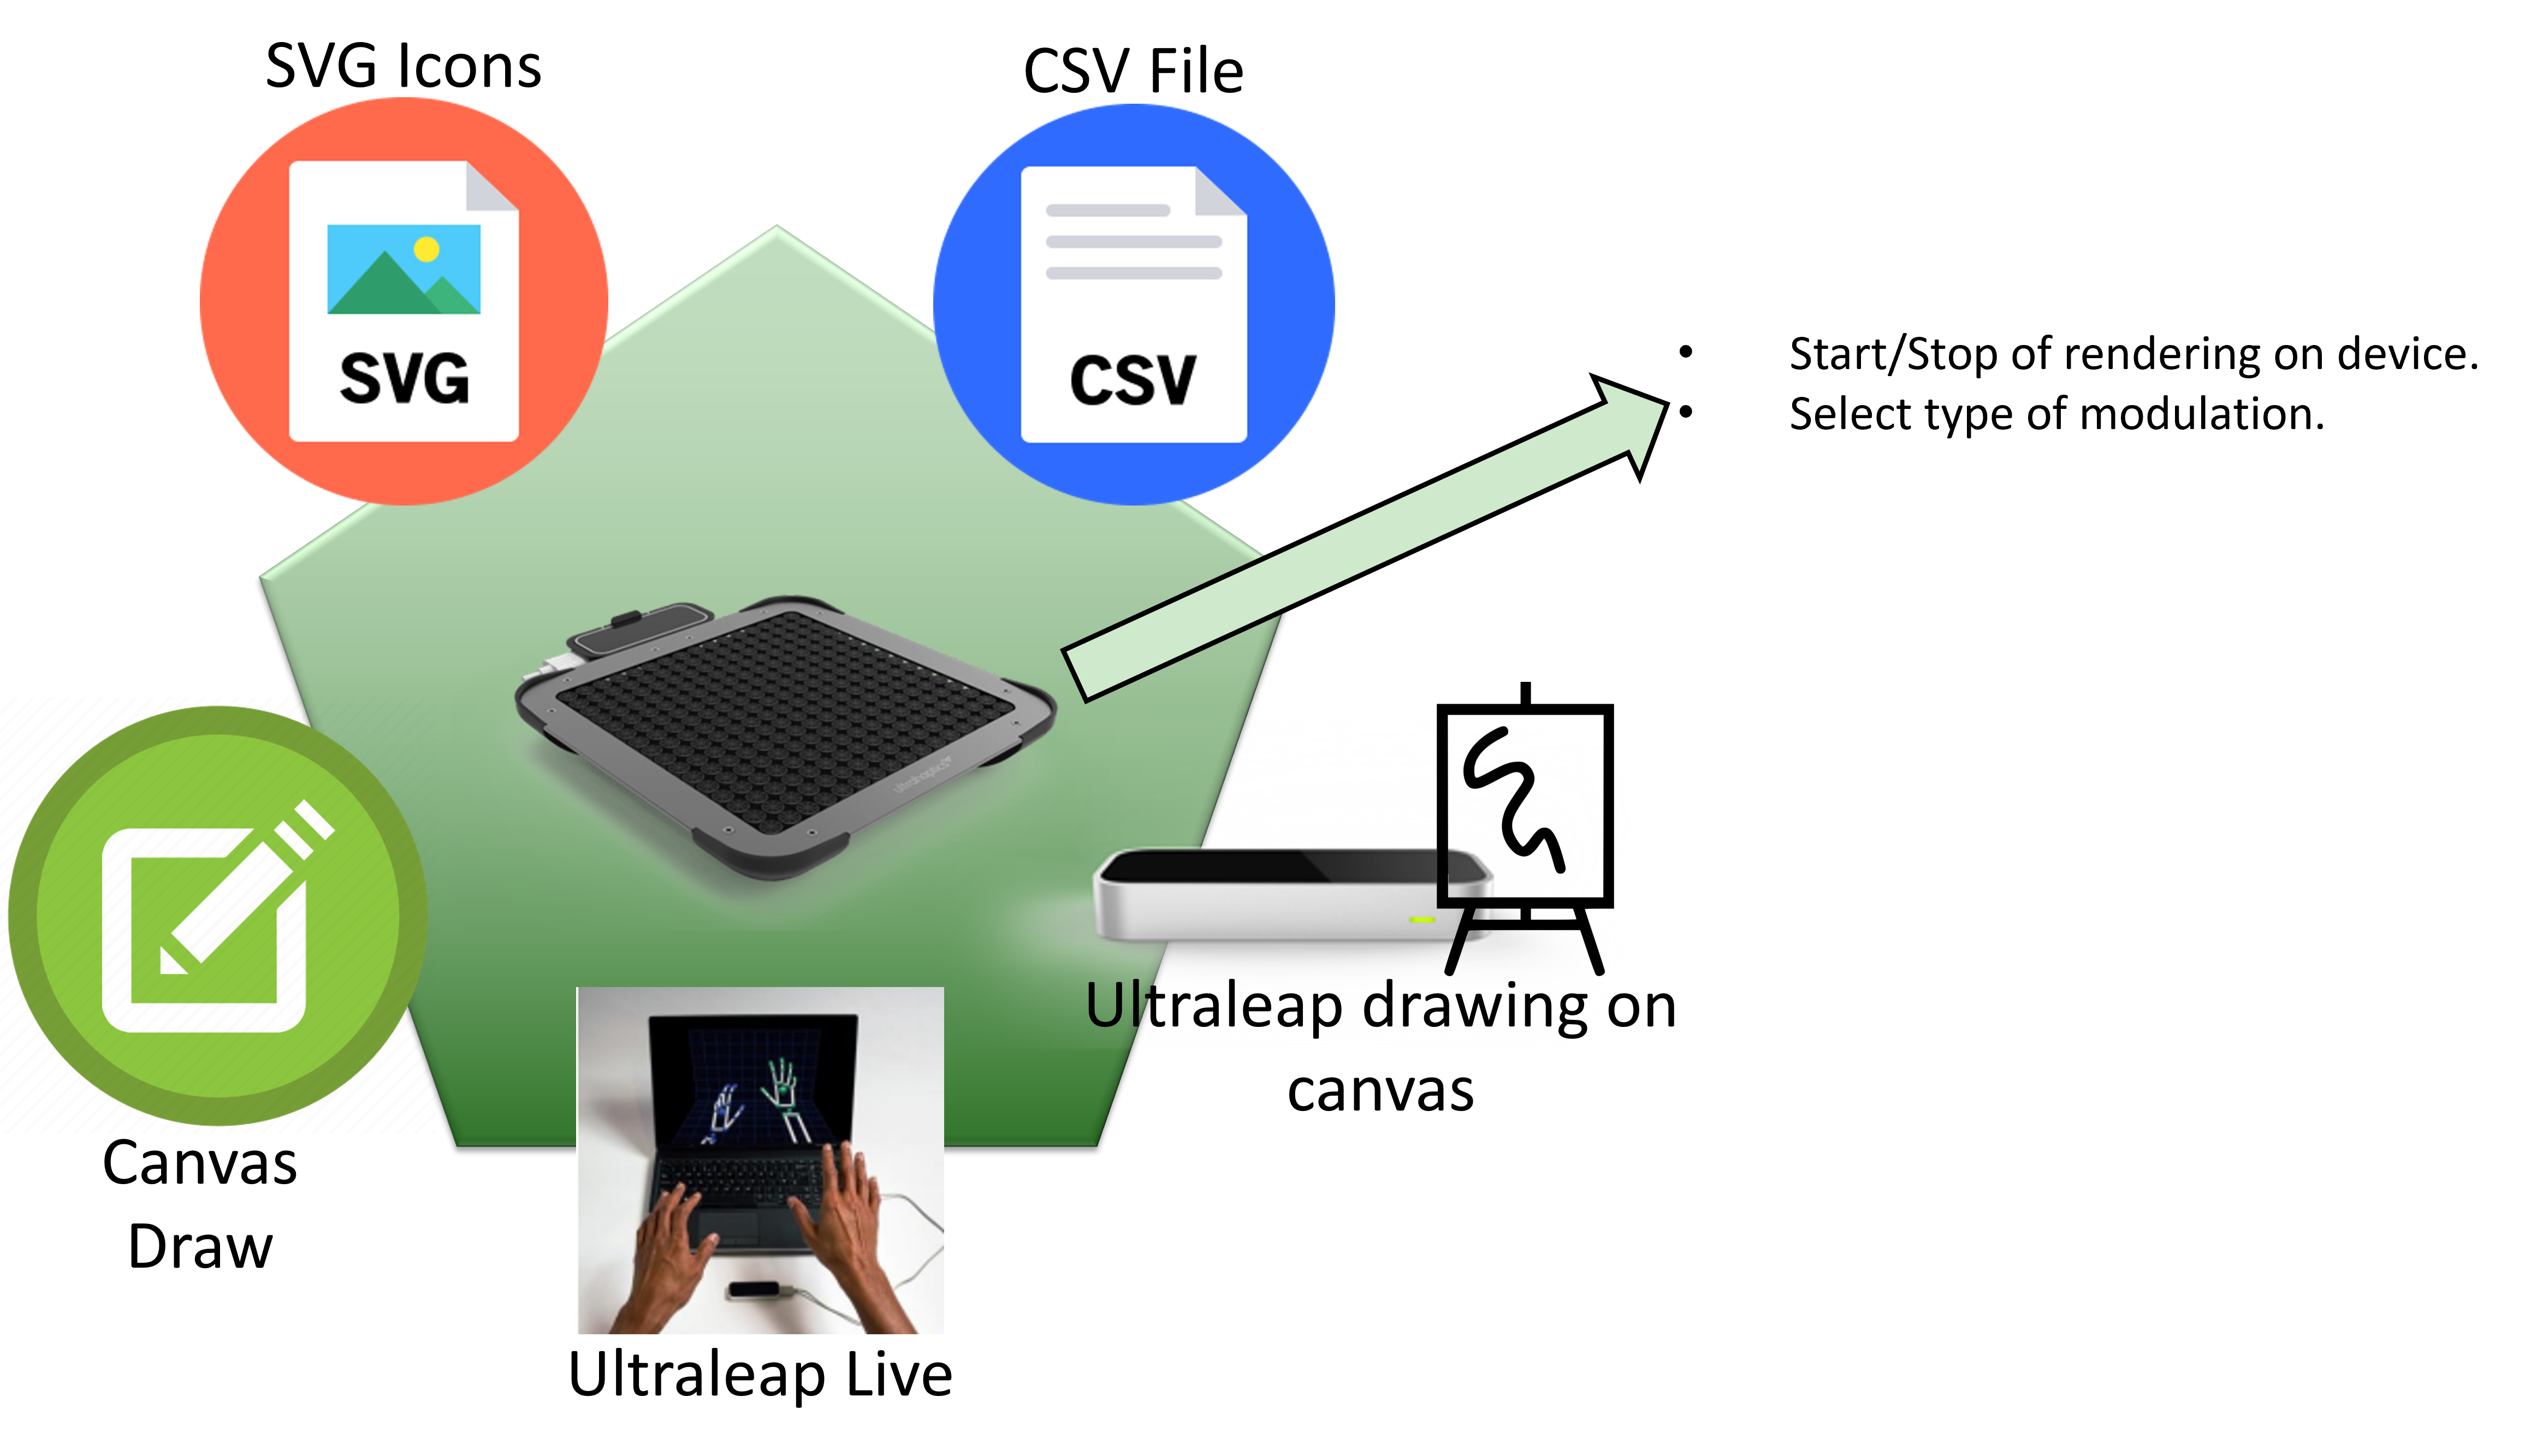
\includegraphics[width=\textwidth]{gfx/Features.png}
	\caption{Figure: Features of the application}
	\label{fig:features}
\end{figure}
The features that are supported in the application are categorized in three part: \\[2mm]
a) Output: Ultrahaptics rendering.\\
b) Inputs: multiple types of inputs supported.\\
c) Controls: how user can control rendering.\\[2mm]

% according to the ultrahaptics device
% which should not be over . However, in CSV file the unit is considered to 
% be in meters. For eg. the coordinate (4,5) mm should be 0.004, 0.005 in CSV file.
\section{Output}
Since this application revolves around one major output, it is important to mention 
the output in the beginning. The single output of the application is 
the custom dynamic shape to be rendered/emitted by the ultrahaptics device. 
Since, the device has limited size each input coordinate/s should  be scaled accordingly.

\section{Inputs}
Multiple types of inputs are accepted in the application and tabs are 
created for different inputs, these tabs can be seen in fig 3.2:
\begin{figure}[htb]
	
\includegraphics[width=140mm]{gfx/tabs.jpeg}
	\caption{Tabs in WebApp}
	\label{fig:features:tabs}
\end{figure}


\subsection*{CSV File}
A CSV file which has the coordinates of points in an x,y plane in column family. 
It can be uploaded in File tab. It is assumed that 
the coordinates are mentioned in meters. But since the size of ultrahaptics is 16mm $\times$  16mm
the values in CSV are expected to be in that range. For eg the coordinate (4,5) mm 
should be 0.004, 0.005 in CSV file. An example of the csv input plotted on an xy plane 
can be seen in figure 3.3 only for the visual purpose. \\
\begin{figure}[htb]
	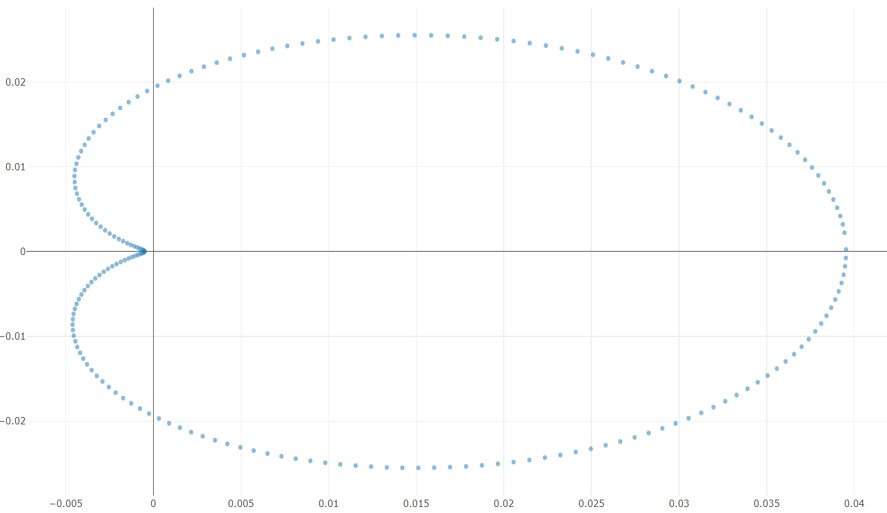
\includegraphics[width=80mm]{gfx/csvinput.jpeg}
	\caption{Example csv Plotted on xy plane}
	\label{fig:features:csvinput}
\end{figure}
In other forms of inputs to the application, the 
coordinates are scaled and centered to size of the Ultrahaptics device by the application. 
However in csv input, it is assumed that the coordinates are scaled and centered.
As soon as the user clicks on the render button the coordinates are 
transferred to the Ultrahaptics device and it starts rendering.


\subsection*{SVG File}
An SVG is also accepted as input format in the same tab as csv. 
As soon as the user uploads the SVG its thumbnail is shown on the 
same page to confirm the visibility. 
SVG coordinates are then communicated to the ultrahaptics device for that shape to
be emitted after user clicks on render button. 


\subsection*{Canvas Draw}
This feature can be accessed under Canvas tab. A HTML 
canvas is provided in which user can draw basic shapes and patterns. 
The coordinates from the canvas is then communicated to the backend and 
rendered on the ultrahaptics device. 

\subsection*{Ultraleap Live}

Ultraleap[ultraleap.com] is an advanced hand tracking  hardware sensory device that accepts hand and 
finger gestures as input, similar to a mouse, but without the need for physical contact.
It is is a tiny USB peripheral device that is meant to be put on a physical desktop 
with its face forward. It's also compatible with virtual reality headsets. 
The gadget observes a roughly hemispheric region to a distance of about 1 meter using 
two monochromatic infrared cameras and three infrared LEDs\cite{s130506380}. The LEDs emit patternless 
infrared light, and the cameras capture almost 200 frames per second of reflected data\cite{leap-controller}. 
This is then transferred to the connected computer via USB connection, where it is processed 
by the company's proprietary hidden code, synthesizing 3D position data by comparing the 
2D frames recorded by the sensors. \\

\begin{figure}[htb]
	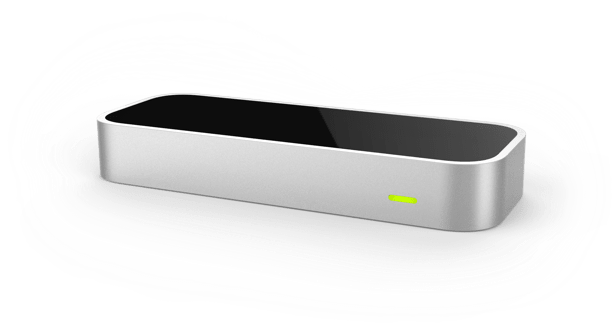
\includegraphics[width=80mm]{gfx/motion-leap.png}
	\caption{Leap motion controller}
	\label{fig:features:csvinput}
\end{figure}
We consume the data provided by the leap controller and mimic the motion, movement and direction of 
moving index finger on the ultrahaptics board. Another requirement of the feature 
is also an ultraleap device connected and 
setup on the system where the webpage is accessed. This feature is accessible in the tab leap 
live. \\

\subsection*{Ultraleap Canvas Draw }
Similar to the ultraleap live user can draw shapes on a canvas provided in WebApp
 using the leap motion controller. As soon as the user clicks on render button the 
 shape is rendered on ultrahaptics board. \\[4mm]


\textbf{Note:} To provide input through leap motion controller device, click on the Start Leap 
button provided in our WebApp and then do the click/tap gesture by your index finger above 
Ultraleap motion controller device. 
After that you will get a banner notification that the system is tracking your finger.\\ 
Do the similar gesture to stop the tracking.\\


\section{Controls}
Some basic controls are also provided in the applications where user can select and 
control other factors, such as:\\
\subsection*{Stop button:} 
On top right of our WebApp a stop button is provided, the rendering on the ultrahaptics 
device can be stopped anytime using this button.\\
\subsection*{Selecting type of rendering:}
On top left of the webapp there is a dropdown select. Here user can switch between
Amplitude Modulation or Time Point streaming for rendering. Once user has selected 
AM, and now wants to observe TPS, rendering has to be stopped by the stop button
before switching.

	% INCLUDE: system
% !TEX root = ../The-Haptic-Printer.tex
%
\chapter{Architecture}
\label{sec:architecture}

\cleanchapterquote{Any application that can be written in JavaScript, will eventually be written in Javascript.}{Jeff Atwood}{Code Horror (blog)} 

This section describes the usage and mapping of hardware and software of this application. This section 
will clear out some questions about the application like, how the application
is consuming the inputs? How the application is transforming input to the desired output? 
How are the middle layers processing the data? Including some other questions about communication of different components.
The aim of this section is to explain in detail the architecture of the application and flow of features. This will also 
explain the requirements to execute the application on local system.

\begin{figure}[htb]
	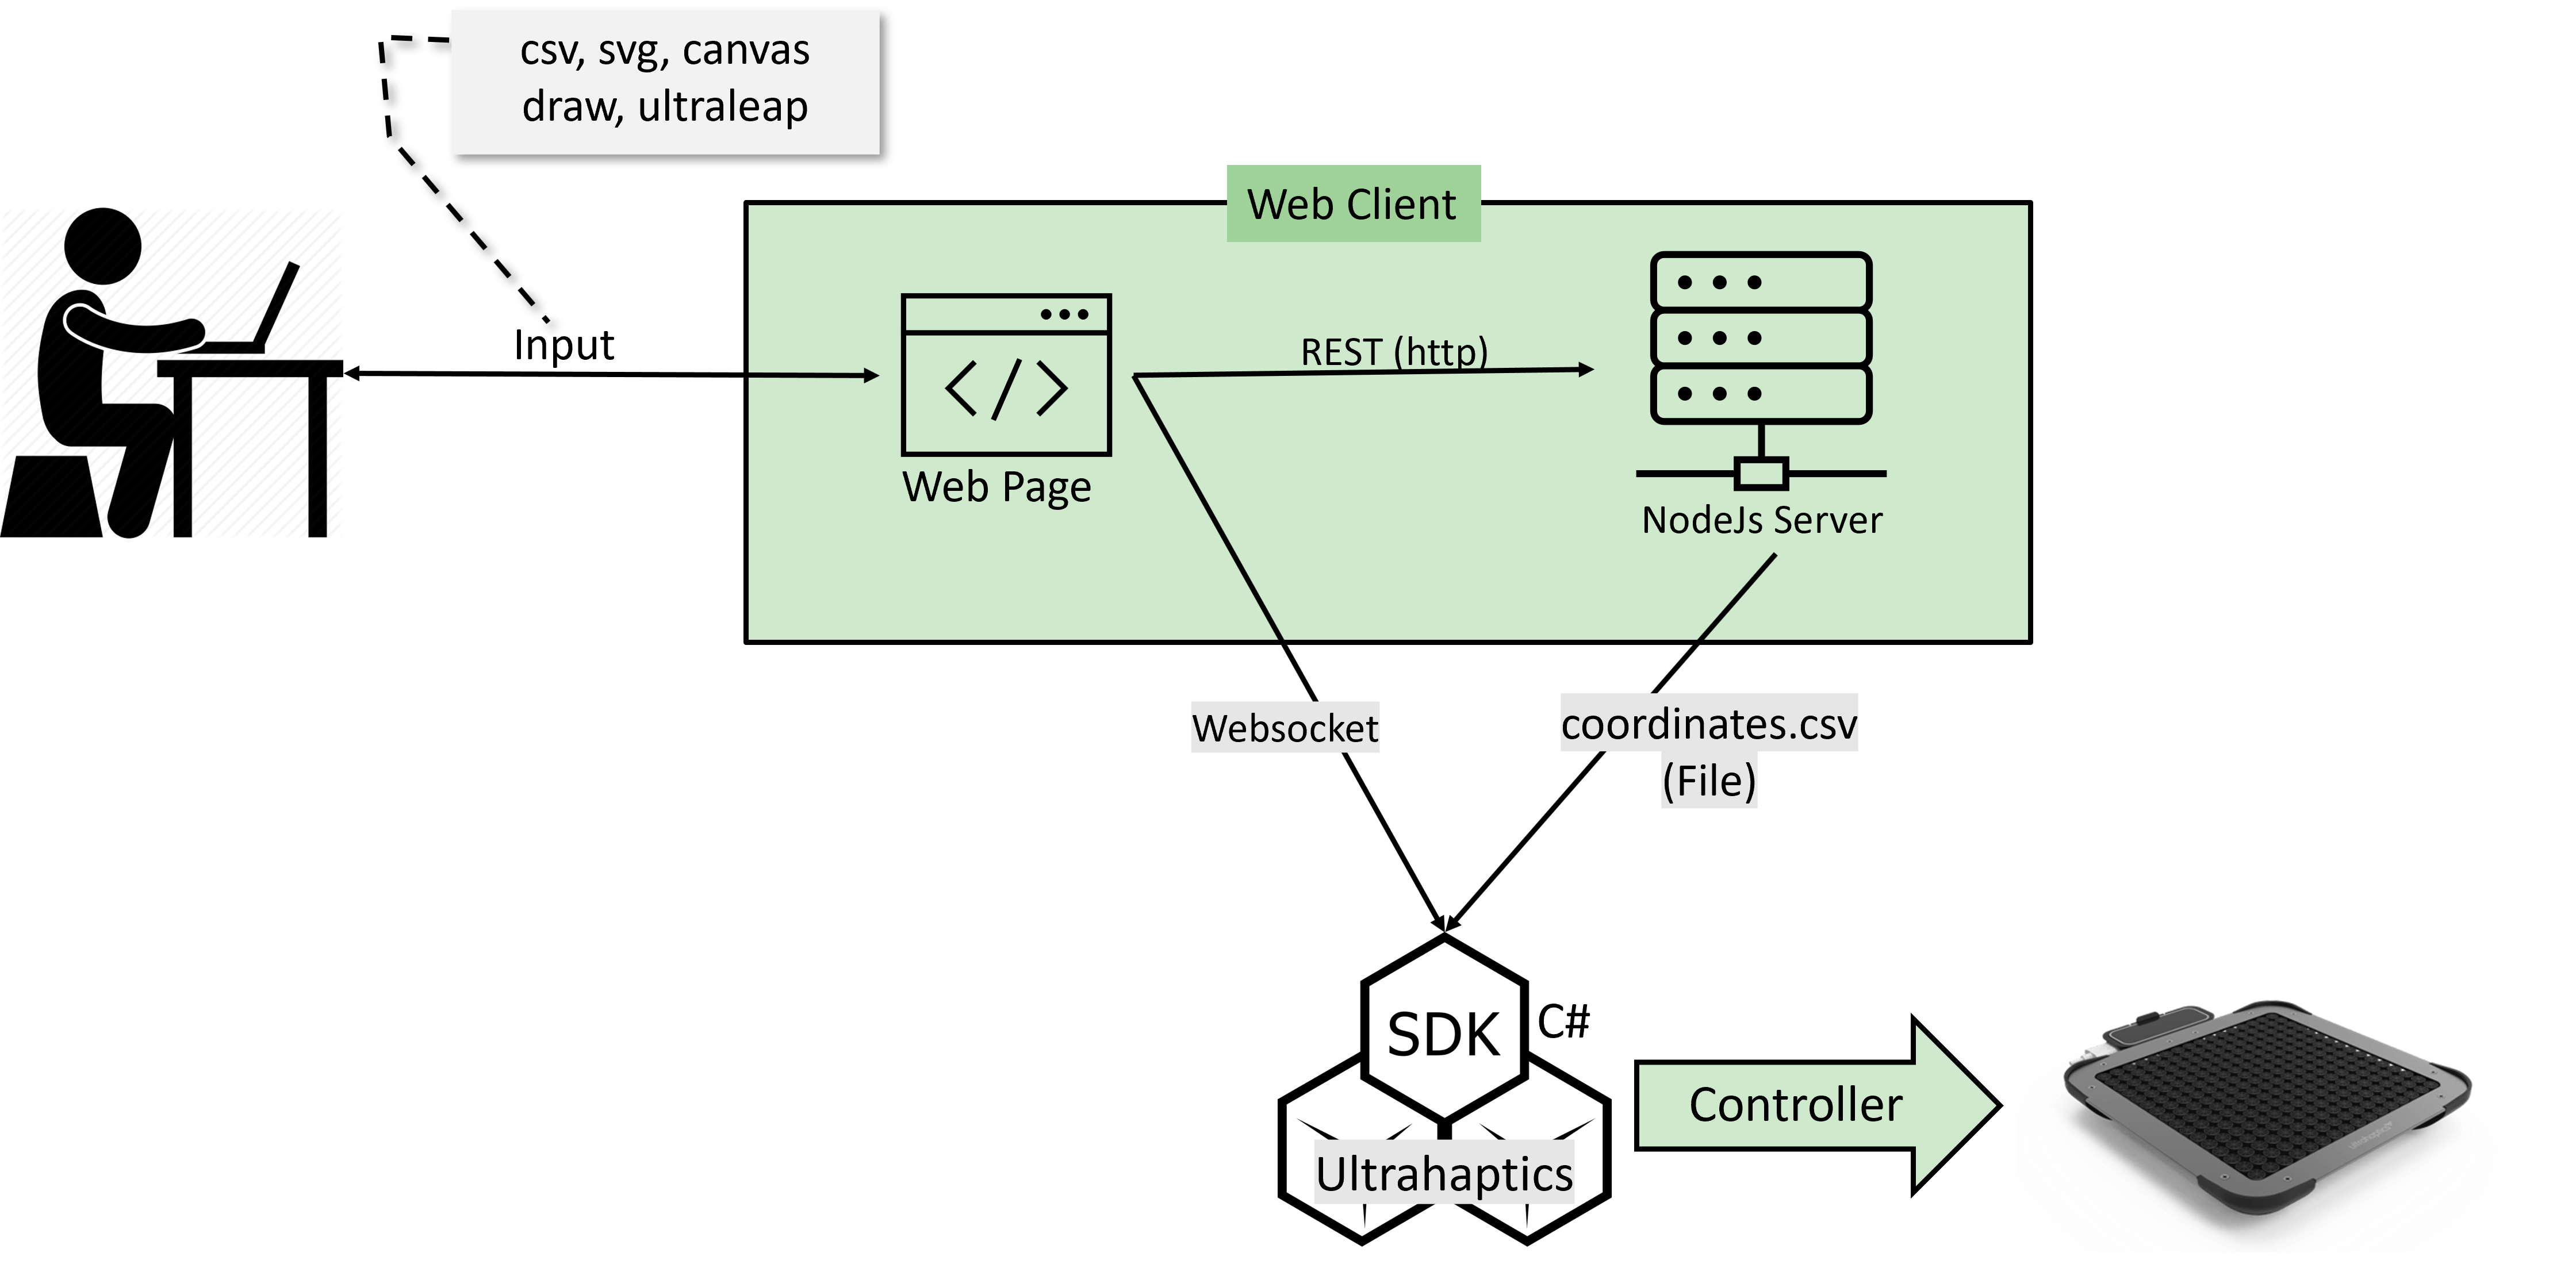
\includegraphics[width=\textwidth]{gfx/Ultrahaptics-custom-architecture}
	\caption{The Haptic Printer (Application architecture)}
	\label{fig:architecture:overall architecture}
\end{figure}


As seen in the architectural diagram Fig 4.1 there are multiple components of
 the application, from user 
input to ultrahaptics device to the communication through websocket and REST. 
The components are mentioned in detail below:\\

\section{Frontend}
The front end of the application is the web. The web application is built in 
vanilla-JS served over a nodeJs Server. However, for compiling 
js code for browser babeljs\cite{babel7.15} is used.

\subsection*{The WebApp and Inputs}
The webpage is responsible for taking multiple inputs from the user and start and stop Ultrahaptics device.
The inputs are in form of the canvas draw, SVG icons, CSV file with (x, y) coordinates, Ultraleap inputs. 
The web page is responsible to scale and center the coordinates (according to x/y plane) taken from multiple input types to the 
Ultrahaptics dimensions and units.\\
In case of SVG some more processing is required. Since, there is no direct feature provided by the 
browser to extract the coordinates from an SVG. The code written for this is a custom implementation inspired from a 
spotify tool\cite{spotify-coordinator} which is under Apache license 2.0 . After extracting the coordinates from the 
given input the coordinates are scaled according to the output device and sent to the backend server in NodeJs, 
the processing in the nodeJs is explained in the section backend. \\
After, the successful response from the Node Server the front end is also responsible to communicate to the 
Ultrahaptics SDK implementation to start and stop the Ultrahaptics rendering.

\section{Backend}

The Backend is further divided into two parts. The First, is the Node Js Server. Second is, the system implementation 
in C-sharp, which is responsible to control and render shapes in Ultrahaptics device. \\[4mm]
\subsection*{NodeJs Server} 
The functionality of nodeJS server is minimal. It hosts the WebApp at localhost:3000 in its root and also 
consumes the scaled coordinates from the WebApp. After getting the coordinates it creates a CSV file and writes 
all the coordinates in a csv as x,y as two columns. Post this functionality it responds to the webapp with a success message. 
This CSV file is later consumed by the SDK API implementation to render it on Ultrahaptics device.\\[4mm]

\subsection*{The SDK extension: Ultrahaptics API's} 
Ultrahaptics SDK\cite{Ultrahaptics-APIs} has provided some of the classes to manipulate the control points, 
intensity and how the emitter will respond to the control points and positions provided to it. We built a 
system using these API's to continuously render custom points and shapes provided. 
All the previous implementations and tests we found were for a shapes which were pre defined in the code 
and it was a challenge to dynamically change the emitter points at a given time.  \\
This part of the system implements two types of rendering Amplitude Modulation(AM) and Time Point Streaming(TPS).
Both the implementations consumes dynamic inputs and detail explanation of how it is implemented 
can bee seen below in code documentation in Files AM.cs and TPS.cs. The choice of rendering type 
between AM and TPS can be selected from the WebApp. \\
The system also implements a websocket for communication which will be discussed further. 

\section{Communication}
\subsection*{Websocket}
The websocket communication happens between the web app and Csharp Ultrahaptics system to consume API's.
Where Csharp implements the websocket server $UltrahapticsOrchestrator.cs$ and webapp implements the 
websocket client $cswebsocket.js$. The webapp sends a message to backend system to start or stop the
Ultrahaptics device rendering, using websocket. It also sends what type of rendering to use(AM or TPS). the websocket 
communication message is in JSON format and an example message can be seen below.
\begin{figure}[htb]
	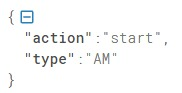
\includegraphics[width=40mm]{gfx/jsonstart.jpeg}
	\caption{Json example to start AM rendering}
	\label{fig:architecture:json}
\end{figure}

\subsection*{REST}
The REST communication in between the webapp and the NodeJs server. After the input processing in the webapp the coordinates are sent to 
the NodeJs using this REST channel at $localhost:3000$.  
\subsection*{CSV file I/O}
After the NodeJs server receives the coordinates, the coordinates are written to a csv file in the column format. 
Column names (x,y). These coordinates file is picked up by the Ultrahaptics API implementation system, and uses these 
coordinates to render the mentioned points.


% !TEX root = ../The-Haptic-Printer.tex

\chapter{Validation}
\label{sec:validation}

After the development of our web application it was time for validation to check how the custom shapes are being rendered from the Ultrahaptics device. In order to validate our rendered shapes we shortlisted three different techniques which are explained in detail in the following sections.


\section{Ultraviz tool}
\label{sec:validation:ultraviz}

The Ultraviz is a tool developed by Ultraleap \cite{ul}\cite{ultraviz} to visualize control points that are being rendered by the Ultrahaptics device in a three dimensional space. It helps the developer to understand how the rendering is happening visually. With the help of this tool we tried to analyse the different rendering techniques like AM and TPS with different kind of inputs i.e, CSV, SVG, drawing on canvas, live leap motion and drawing on canvas with the help of leap motion. 

The following are the various kinds of inputs we tried to render:

\textbf{Note:} Since the images are screenshots of the Ultraviz visualization tool, we cannot see all the control points being rendered in the image as it is moving at a high speed.

1. Read CSV file feature:
\begin{figure}[H]
	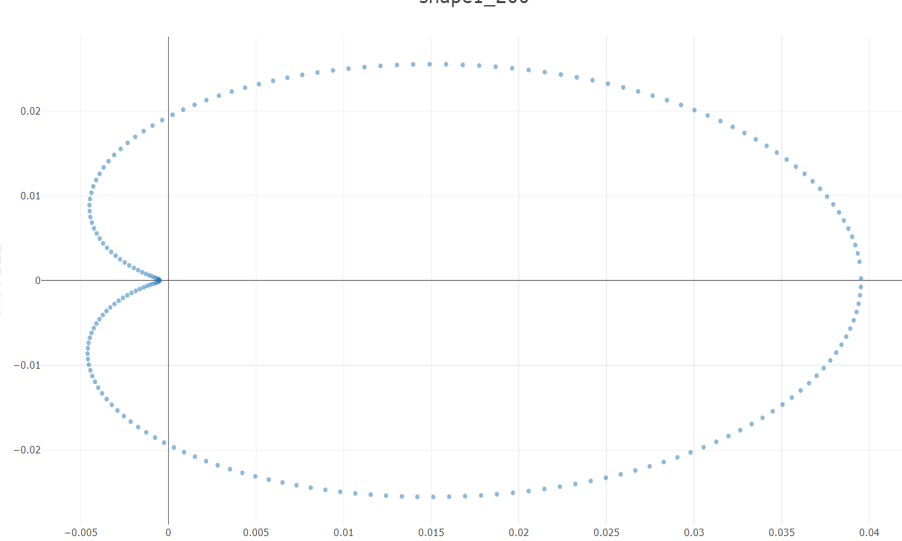
\includegraphics[width=\textwidth]{gfx/Read CSV Image.png}
	\caption{CSV Plot of a custom shape}
	\label{fig:validation:csv}
\end{figure}

The x and y coordinate values are read from a CSV file and the plot is as shown in Fig 5.1.
This plot will be rendered in the Ultrahaptics device. Fig 5.2 (a) represents the CSV plot being rendered on Ultrahaptics using AM technique and Fig 5.2 (b) represents the same CSV plot in TPS technique. 

\begin{figure}[H]
	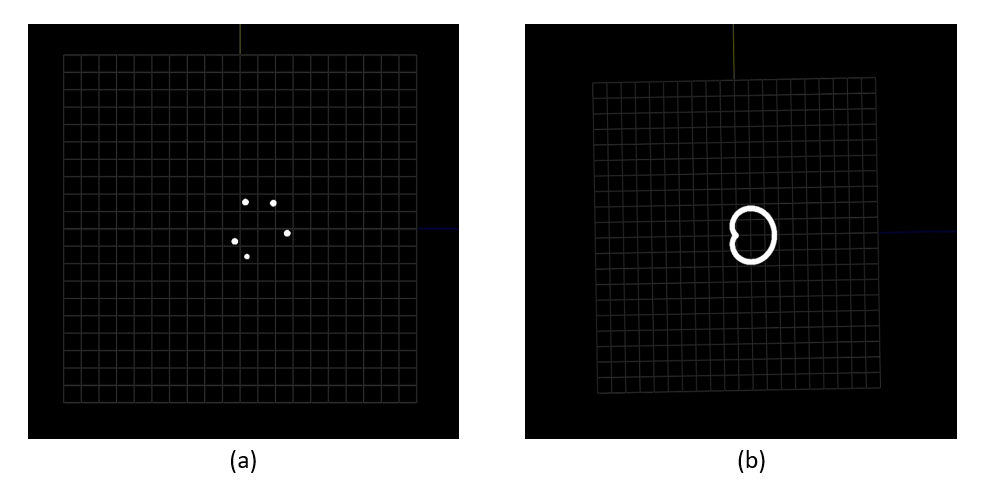
\includegraphics[width=\textwidth]{gfx/read_csv_rendering.png}
	\caption{(a) Ultraviz visualization of CSV plot in AM and (b) TPS technique}
	\label{fig:validation:csv_am}
\end{figure}

2. SVG file input feature:
\begin{figure}[H]
	\includegraphics[width=\textwidth]{gfx/SVG Input.png}
	\caption{SVG input shapes (a) Arrow Down (b) WiFi (c) Square}
	\label{fig:validation:svg}
\end{figure}

\begin{figure}[H]
	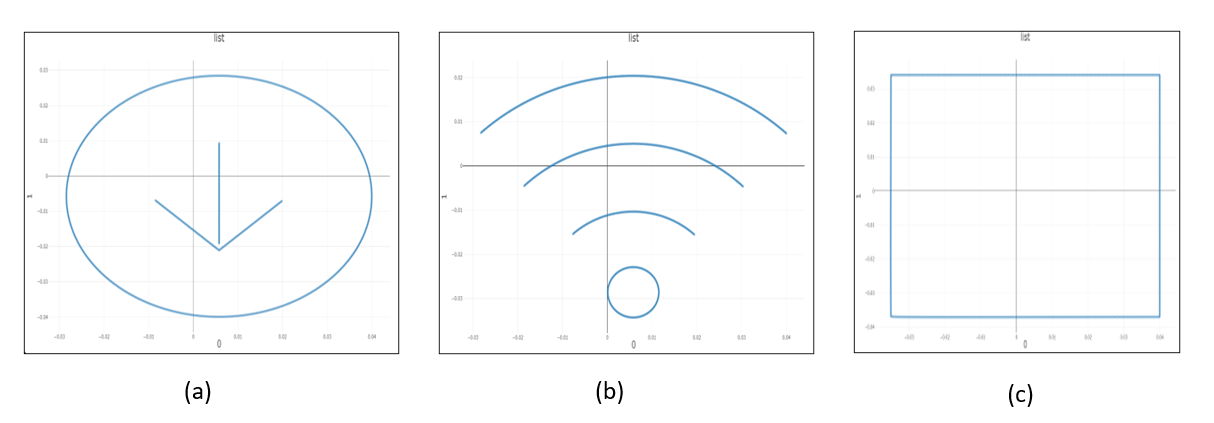
\includegraphics[width=\textwidth]{gfx/svg_plot.png}
	\caption{SVG plot of input shapes (a) Arrow Down (b) WiFi (c) Square}
	\label{fig:validation:svg_plot}
\end{figure}

Fig 5.3 depicts the various SVG files used to render on Ultrahaptics device. Once the SVG files are uploaded  it is converted to x and y coordinate system with specific number of points. Fig 5.4 shows the different xy plot of the SVG files uploaded.
 

\begin{figure}[H]
	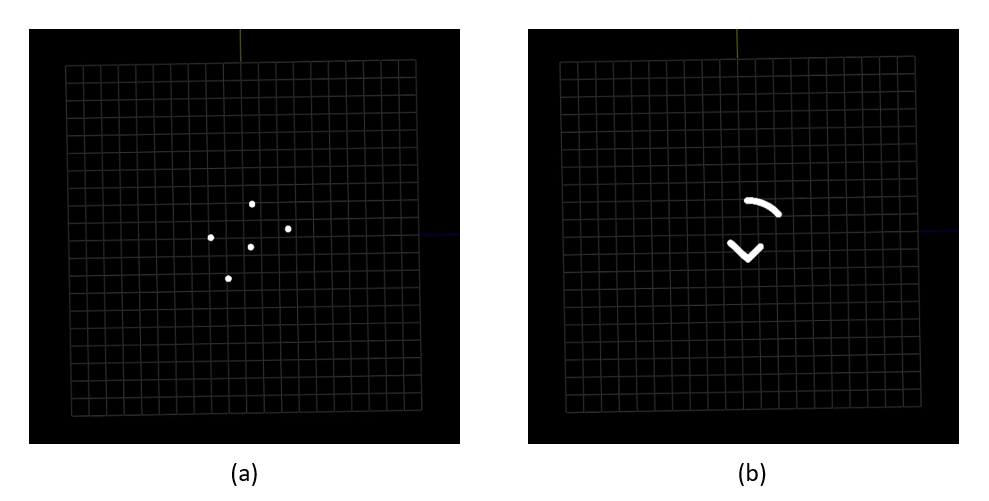
\includegraphics[width=\textwidth]{gfx/svg_ad.png}
	\caption{(a) SVG rendering of arrow down in AM (b) SVG rendering of arrow down in TPS}
	\label{fig:validation:svg_ad}
\end{figure}

\begin{figure}[H]
	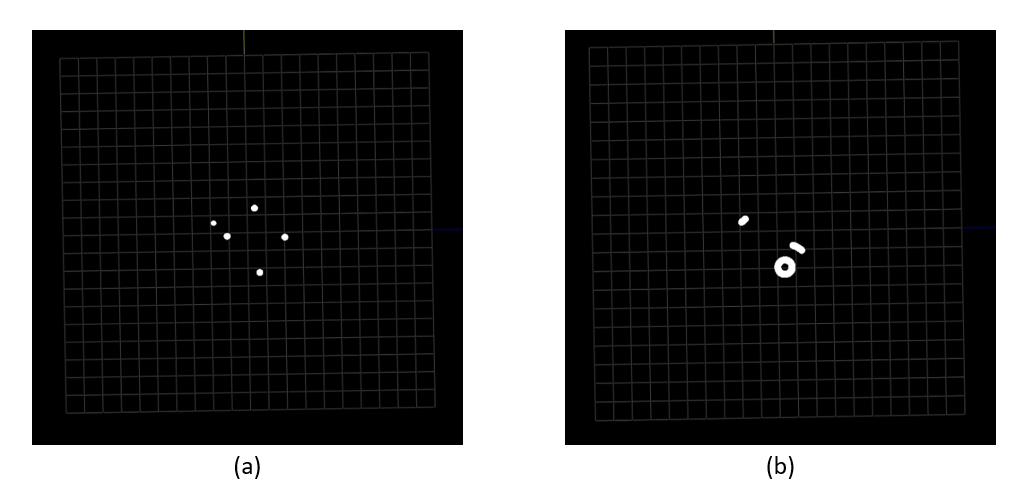
\includegraphics[width=\textwidth]{gfx/svg_wifi.png}
	\caption{(a) SVG rendering of WiFi in AM (b) SVG rendering of WiFi in TPS}
	\label{fig:validation:svg_wifi}
\end{figure}

\begin{figure}[H]
	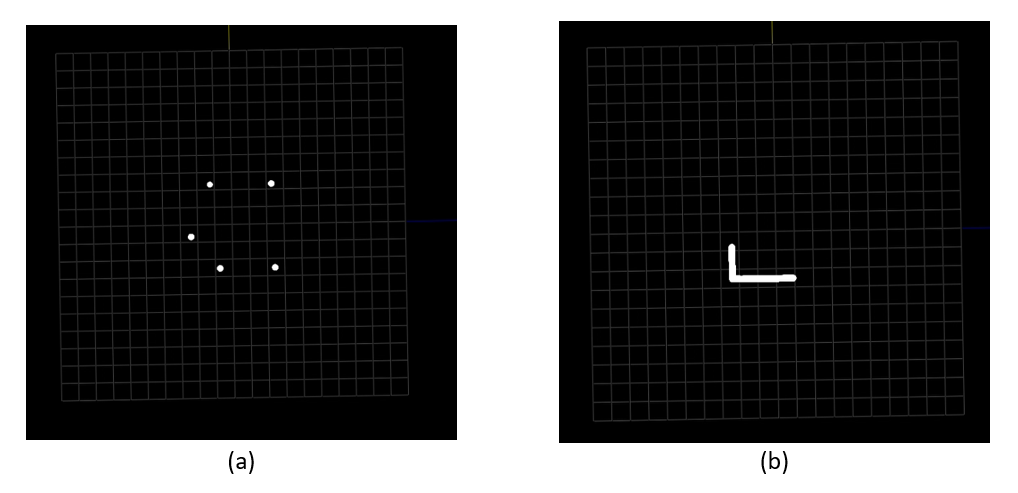
\includegraphics[width=\textwidth]{gfx/svg_sq.png}
	\caption{(a) SVG rendering of square in AM (b) SVG rendering of square in TPS}
	\label{fig:validation:svg_sq}
\end{figure}

Fig 5.5, Fig 5.6, Fig 5.7 displays an image of Ultraviz tool rendering the SVG inputs arrow down, WiFi and square in AM and TPS technique respectively.

3. Drawing on canvas:

The user can draw the shapes on the given HTML canvas using mouse. Fig 5.8 (a) shows a user drawn circle shape and Fig 5.8 (b) shows an plot of the user shape represented in x and y coordinate which will be eventually rendered on Ultrahatics.

\begin{figure}[H]
	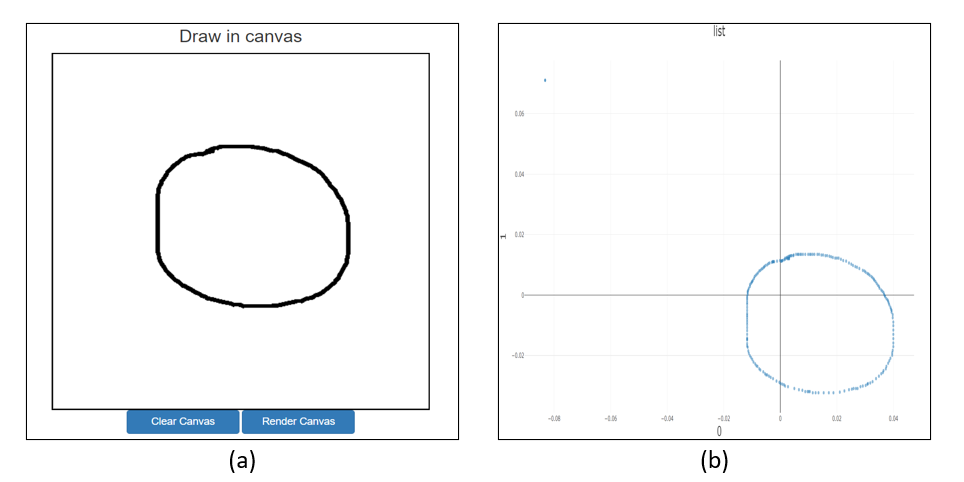
\includegraphics[width=\textwidth]{gfx/canvas input.png}
	\caption{(a) User drawn circle shape on HTML canvas (b) XY plot of the given user shape}
	\label{fig:validation:svg_sq_tps}
\end{figure}

Fig 5.9 (a) depicts the rendering of custom user shape in Ultraviz in AM and Fig 5.9 (b) depicts the same in TPS technique.

\begin{figure}[H]
	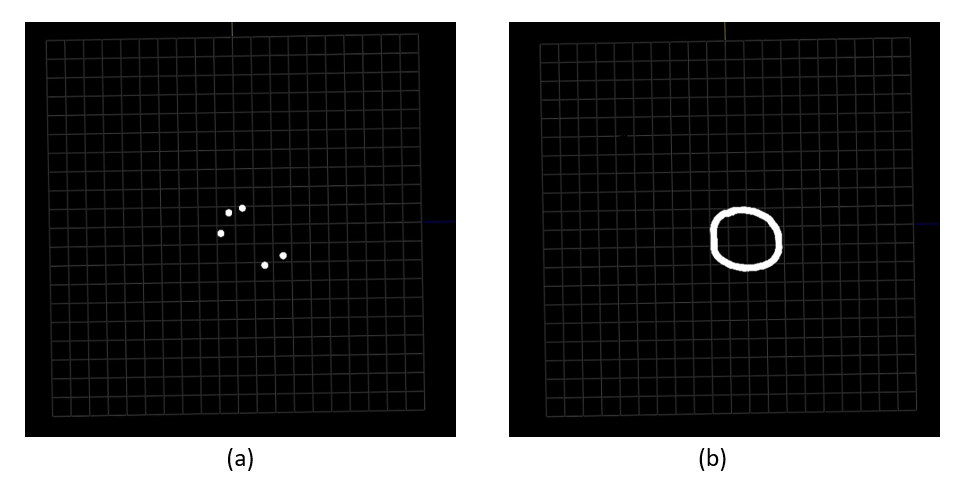
\includegraphics[width=\textwidth]{gfx/canvas_uv.png}
	\caption{(a) User drawn circle rendering in AM technique (b) User drawn circle rendering in TPS technique}
	\label{fig:validation:svg_sq_tps}
\end{figure}

4. Leap Canvas:

Leap canvas is similar to canvas drawing, instead of using mouse as a drawing tool here we use our index finger and with the help of Ultraleap leap motion device we draw on the canvas. Later the canvas drawing is converted to xy plot and then rendered on the Ultrahaptics device.

5. Leap Live:

Leap live uses the Ultraleap leap motion device to track our index finger and the same point is being rendered live on the Ultrahaptics device. The control point moves in the direction of the Ultraleap leap motion hand input.

\section{Cross validation and observation from developers}
\label{sec:validation:cross validation and observation from developers}

In order to further validate our project we conducted a short study between the authors of this project where we chose three different shapes i.e, square, circle and triangle and decided to guess the shape in various different techniques. In the first study we did not tell the observer on the Ultrahaptics which all shapes where there in the study and the observer guessed everything as circle. 

Later in the second study, we informed the observer the available shapes and then performed the study. We conducted the study mutually between us and below are the results:
Square shape was easily identified by both of us in AM technique and both guessed the square shape as circle in TPS technique. Triangle was guessed correctly in both the techniques. Circle was guessed correctly in TPS technique and one observer reported circle as triangle in AM technique. \\
Hence, from this short observation it was concluded that basic shapes if known to the subject in advance are recognized in a better manner.

Below in Fig 5.10 you can see all the results summed up in a table. 

\begin{figure}[H]
	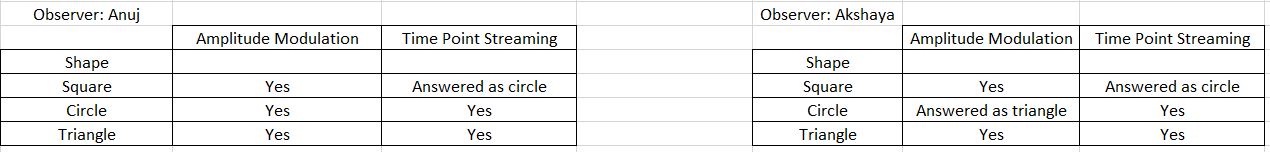
\includegraphics[width=150mm, height=25mm]{gfx/user_study_result.png}
	\caption{Results of validation between the authors of the project}
	\label{fig:validation:svg_sq_tps}
\end{figure}


\section{Oil bath}
\label{sec:validation:oilbath}

We also came across a technique where the rendering can be projected on an oil bath set-up to visualize how the inputs are being rendered on the user palm \cite{oil}. This experiment was a guided setup by the ultrahaptics support team. The step by step guide to set up the environment is as follows:

1. The Ultrahaptics device is suspended approximately 15cm above the oil bath using a robotic arm. There is no need to use the Leap Motion so the cradle can be separated. 

2. The oil is between 2 and 5mm deep. There is a purpose built perspex tank of 30 centimetres for the experiment. The oil must have the correct consistency and viscous enough to show dispersion, fluid enough to be responsive. We have found that a 50:50 mix of olive oil and pumpkin seed oil give good results. 

3. The oil bath must be raised approximately 3 cm above a white surface. We used legos for this purpose and used two A3 sheets of paper as a white surface.

4. Light with a single, small, bright light source from above or to an angle to project the shadow of the distorted surface on to the oil. There is a small, LED light available on an adjustable stalk. Place it between top of tank and perspex holder, with light covering as much of oil as possible. The light must be bright enough to reflect onto a wall and the room must be as dark as possible to achieve the best affect.

Fig 5.11 and Fig 5.12 show the experiment setup of oil bath. 

\begin{figure}[htb]
	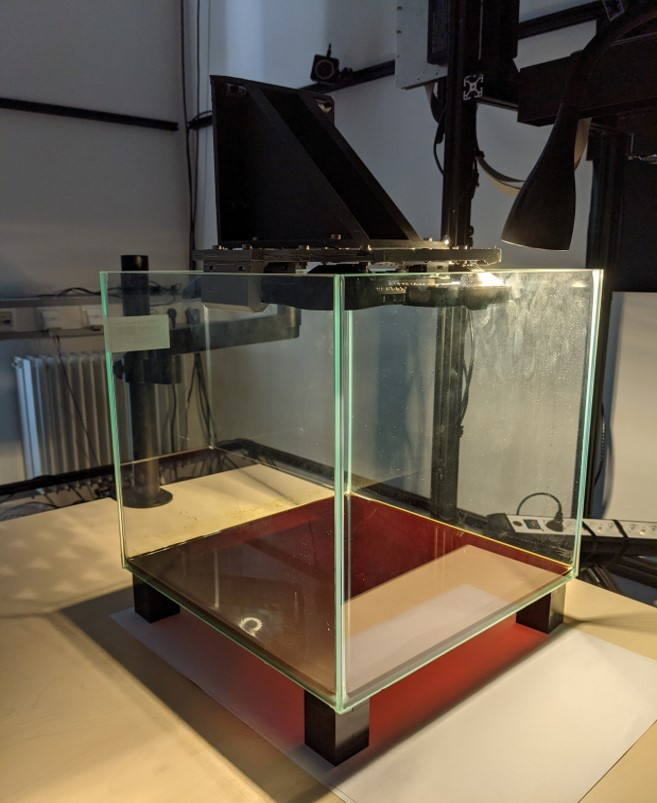
\includegraphics[width=\textwidth]{gfx/oilbath1.jpg}
	\caption{Overall oil bath setup}
	\label{fig:validation:oil_bath1}
\end{figure}

\begin{figure}[htb]
	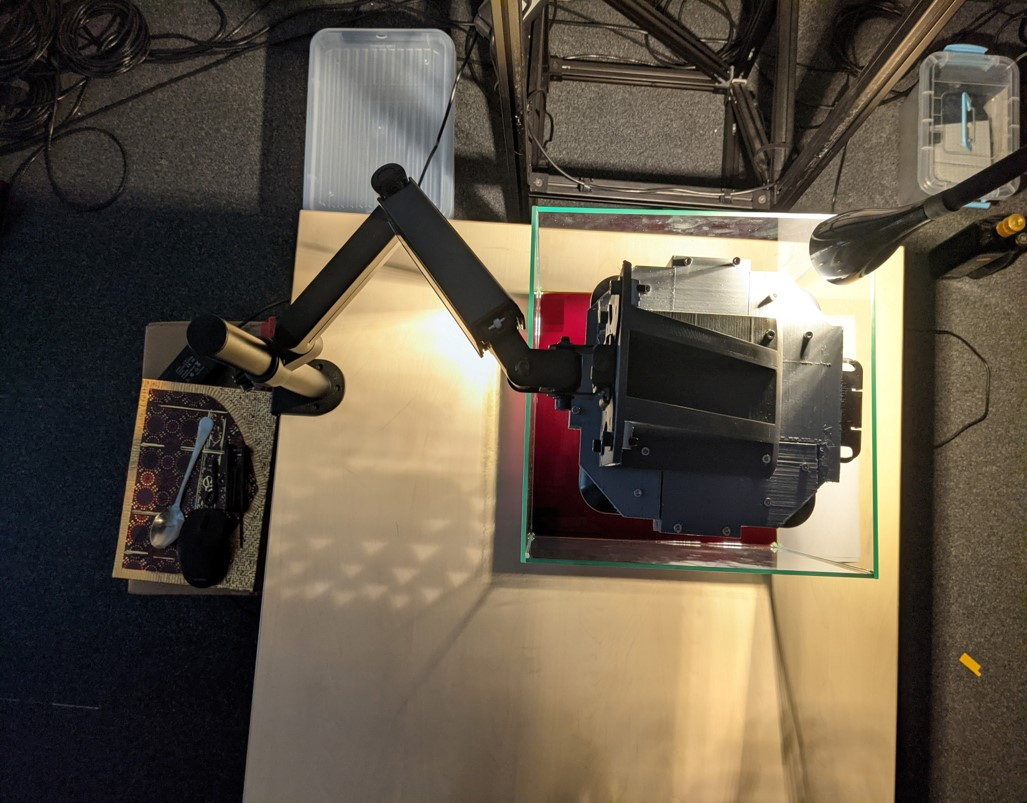
\includegraphics[width=\textwidth]{gfx/oilbath2.jpg}
	\caption{Top view of oil bath setup }
	\label{fig:validation:oil_bath2}
\end{figure}
% !TEX root = ../The-Haptic-Printer.tex
%
%************************************************
% Declaration
%************************************************

\chapter{Conclusion}
\label{sec:conclusion}
After finishing the project and observing multiple shapes using different types of 
rendering methods like AM and TPS, we collectively came to a conclusion that basic primitive geometric
shapes(square, circle triangle, etc) are better recognized in Amplitude Modulation. 
Pointer movement on hand gesture using ultra leap, the feature that we call "Leap Live" 
showed the best results in recognition of movement and directions. \\[2mm]
We also wrote a test script to slow down the pointer movements on the corners of a square and triangle, 
and concluded that corners if rendered with slow pointer movement are recognized a bit easier. The final 
conclusion was that for Ultraviz and oil bath experiment TPS looks better visually. 
However, for hand sensation AM feels better if rendering with varying intensity and frequency.

%*****************************************
%*****************************************

% !TEX root = ../The-Haptic-Printer.tex
%
%************************************************
% Declaration
%************************************************

\chapter{Future Work}
\label{sec:futurework}
The future work relating to this project would be to implement a new method of 
rendering. Where, the system automatically recognizes the curves, corners, 
edges from the varying range of dynamic input and render the same with varying 
intensity and speed dynamically. Also if the input 
is a disjoint figure, like the wifi logo as shown in fig. 5.3(b) and 5.3(b) it is 
better to create different control point for different disjoint lines/curves.\\
To include DTP method mentioned by Hajas in \cite{Hajas2020} for dynamic shapes.
%*****************************************
%*****************************************
 % INCLUDE: concepts
% !TEX root = ../The-Haptic-Printer.tex

\chapter{Appendix}
\label{sec:documentation}

\section{Source Code}
\label{sec:documentation:source_code}
\textbf{AM.cs}
\lstinputlisting[language=csh]{program/AM.cs}
\textbf{TPS.cs}
\lstinputlisting[language=csh]{program/TPS.cs}
\textbf{UltrahapticsCS\_Controller.cs}
\lstinputlisting[language=csh]{program/UltrahapticsCS_Controller.cs}
\textbf{Utility.cs}
\lstinputlisting[language=csh]{program/Utility.cs}
\textbf{WebsocketOrchestrator.cs}
\lstinputlisting[language=csh]{program/WebsocketOrchestrator.cs}


\textbf{package.json}
\lstinputlisting[language=Plasm]{program/package.json}
\textbf{www}
\lstinputlisting[language=Plasm]{program/www}
\textbf{app.js}
\lstinputlisting[language=Plasm]{program/app.js}
\textbf{index.js}
\lstinputlisting[language=Plasm]{program/index.js}
\textbf{render.js}
\lstinputlisting[language=Plasm]{program/render.js}
\textbf{renderCoordinates.js}
\lstinputlisting[language=Plasm]{program/renderCoordinates.js}
\textbf{index.html}
\lstinputlisting[language=html]{program/index.html}
\textbf{startApp.js}
\lstinputlisting[language=Plasm]{program/startApp.js}
\textbf{pathologize.js}
\lstinputlisting[language=Plasm]{program/pathologize.js}
\textbf{polygonize.js}
\lstinputlisting[language=Plasm]{program/polygonize.js}
\textbf{pathsToCoords.js}
\lstinputlisting[language=Plasm]{program/pathsToCoords.js}
\textbf{leap.js}
\lstinputlisting[language=Plasm]{program/leap.js}
\textbf{leapCanvas.js}
\lstinputlisting[language=Plasm]{program/leapCanvas.js}
\textbf{getTotalLengthAllPaths.js}
\lstinputlisting[language=Plasm]{program/getTotalLengthAllPaths.js}
\textbf{cs\_websocket.js}
\lstinputlisting[language=Plasm]{program/cs_websocket.js}
\textbf{canvas\_script.js}
\lstinputlisting[language=Plasm]{program/canvas_script.js}
\textbf{main.js}
\lstinputlisting[language=Plasm]{program/main.js}











\cleardoublepage

% --------------------------
% Back matter
% --------------------------
{%
\setstretch{1.1}
\renewcommand{\bibfont}{\normalfont\small}
\setlength{\biblabelsep}{0pt}
\setlength{\bibitemsep}{0.5\baselineskip plus 0.5\baselineskip}
\printbibliography[nottype=online]
\printbibliography[heading=subbibliography,title={Websites},type=online,prefixnumbers={@}]
}
\cleardoublepage

\listoffigures
\cleardoublepage

% !TEX root = ../The-Haptic-Printer.tex
%
%************************************************
% Declaration
%************************************************
\pdfbookmark[0]{Declaration}{Declaration}
\chapter*{Declaration}
\label{sec:declaration}
\thispagestyle{empty}

I declare that this project, was solely undertaken by myself. All sections of the report that use or describe an concept developed by another author are referenced. 

\bigskip

\noindent\textit{\thesisUniversityCity, \thesisDate}

\smallskip

\begin{flushright}
	\begin{minipage}{8cm}
		\rule{\textwidth}{1pt}
		\centering Anuj Sharma, \\Akshaya Kumar Krishnappa Ramakrishna
	\end{minipage}
\end{flushright}

%*****************************************
%*****************************************


\newpage

\mbox{}

% **************************************************
% End of Document CONTENT
% **************************************************
\end{document}
